%!TEX root = finalReport.tex
%!TEX encoding = UTF-8 Unicode
%==============================================================================
%\section{Introduction}
Programming directly on a real robot gives us good feedback and it is more impressive
than simulations, but not everybody has possible access to real robots. For this reason,
we have programs that simulate the physical world.\\
The first phase of robot manufacturing is its design and modeling. We can design and model the 
robot using CAD tools such as Solid Works, Blender, and so on. One of the main purposes 
of modeling robot is simulation. The robotic simulation tool can check the critical flaws in the robot design and can confirm the 
working of the robot before it goes to the manufacturing phase.

The virtual robot model must have all the characteristics of real hardware, the shape of robot 
may or may not look like the actual robot but it must be an abstract, which has all the physical 
characteristics of the actual robot. 

If we are planning to create the 3D model of the robot and simulate using ROS, you need to learn about some ROS packages which helps in robot designing. ROS has a standard meta package for designing, and creating robot models called robot model, which consists of a set of packages called urdf, robot state publisher and so on.  These packages help us create the 3D robot model description with the exact characteristics of the 
real hardware.

In this chapter, we will cover the following topics:
\begin{enumerate}
\item ROS packages for robot modeling
\item  Understanding robot modeling using URDF
\item  Creating our URDF model
\item  Watching the 3d model in RVIZ
\item  Making our robot movable
\end{enumerate}

\section{ROS packages for robot modeling}
The way ROS uses the 3D model of a robot or its parts, to simulate them. ROS provides some good packages that can be used to build 3D robot models.\\ In this
section, we will discuss some of the important ROS packages that are commonly used to
build robot models:
\\\\\textbf{robot model}: ROS has a meta package called robot model, which contains important 
packages that 
help build the 3D robot models. We can see all the important packages inside this meta-
package:
\\\\\textbf{URDF}: One of the important packages inside the robot model meta package is urdf. The 
URDF package contains a C++ parser for the Unified Robot Description Format (URDF),
which is an XML file to represent a robot model.
\\\\ We can define a robot model, sensors, and a working environment using URDF and 
can parse it using URDF parsers.
\\We can only describe a robot in URDF that has a tree-like 
structure in its links, that is, the robot will have rigid links and will be connected 
using joints. Flexible links can't be represented using URDF.
\\ The URDF is composed using special XML tags and we can parse these XML tags using 
parser programs for further processing. We can work on URDF modeling in the upcoming 
sections.
\\\\\textbf{joint state publisher}: This tool is very useful while designing robot 
models using URDF.
\\This package contains a node called joint state publisher, which reads the robot 
model description, finds all joints, and publishes joint values to all non fixed 
joints 
using GUI sliders. 
\\The user can interact with each robot joint using this tool and can visualize using 
RViz.
\\While designing URDF, the user can verify the rotation and translation of each 
joint using this tool. 
\\\\\textbf{kdl parser}: Kinematic and Dynamics Library (KDL) is an ROS package that 
contains parser tools to build a KDL tree from the URDF representation. The kinematic 
tree can be used to publish the joint states and also to forward and inverse 
kinematics of the robot.
\\\\\textbf{robot state publisher}: This package reads the current robot joint states 
and publishes 
the 3D poses of each robot link using the kinematics tree build from the URDF. The 3D 
pose of the robot is published as ROS tf (transform). ROS tf publishes the 
relationship 
between coordinates frames of a robot.
\\\\\textbf{xacro}: Xacro stands for (XML Macros) and we can define how xacro is equal 
to URDF plus add-ons. It contains some add-ons to make URDF shorter, readable, and can 
be used for building complex robot descriptions. We can convert xacro to URDF at any 
time using some ROS tools. We will see more about xacro and its usage in the upcoming 
sections.

\section{Understanding robot modeling using URDF}

We have discussed the urdf package. In this section, we will look further at the URDF XML tags, which help to model the robot. We have to create a file and write the relationship between each link and joint in the robot and save the file with the .urdf extension.
\\The URDF can represent the kinematic and dynamic description of the robot, visual representation of the robot, and the collision model of the robot.
\\\\The following tags are the commonly used URDF tags to compose a URDF robot model:
\\ \textbf{link}: The link tag represents a single link of a robot. Using this tag, we can model a robot link and its properties. The modeling includes size, shape, color, and can even import a 3D mesh to represent the robot link. We can also provide dynamic properties of the link such as inertial matrix and collision properties.
\\
The syntax is as follows:
\begin{lstlisting}[language=XML]
<link name="<name of the link>">
    <inertial>...........</inertial>
    <visual> ............</visual>
    <collision>..........</collision>
</link>
\end{lstlisting}

The following is a representation of a single link. The Visual section represents 
the real link of the robot, and the area surrounding the real link is the Collision 
section. The Collision section encapsulates the real link to detect collision before 
hitting the real link.
\begin{figure}[h]
	\centering
	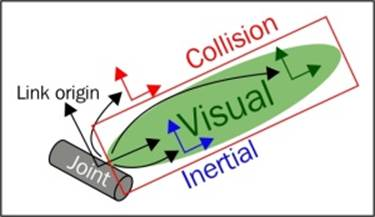
\includegraphics[width=0.7\linewidth]{s1}
	\caption{Visualization of a URDF link}
	\label{fig:s1}
\end{figure}
\textbf{joint}: The joint tag represents a robot joint. We can specify the kinematics and dynamics of the joint and also set the limits of the joint movement and its velocity. The joint tag supports the different types of joints such as revolute, continuous, prismatic,fixed, floating, and planar.

The syntax is as follows:
\begin{lstlisting}[language=XML]
<joint name="<name of the joint>">
  <parent link="link1"/>
  <child link="link2"/>
  <calibration .... />
  <dynamics damping ..../>
  <limit effort .... />
</joint>
\end{lstlisting}
A URDF joint is formed between two links; the first is called the Parent link and the second is the Child link. The following is an illustration of a joint and its link:\\
\begin{figure}[h]
	\centering
	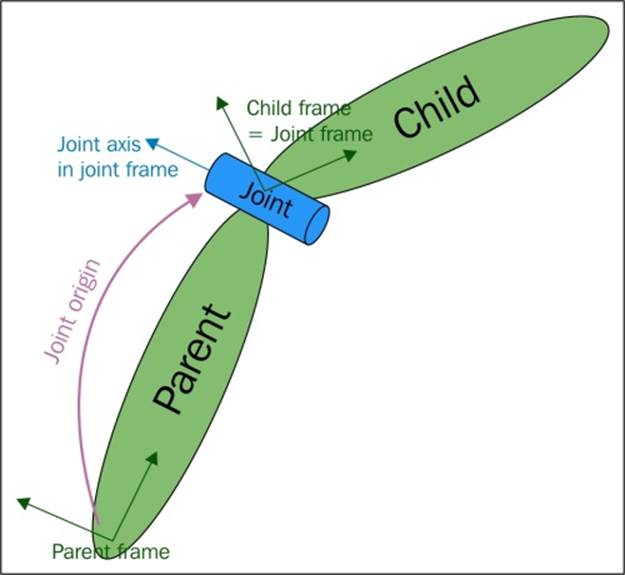
\includegraphics[width=0.6\linewidth]{s2}
	\caption{Visualization of a URDF joint}
	\label{fig:s2}
\end{figure}
\textbf{robot}: This tag encapsulates the entire robot model that can be represented using URDF. Inside the robot tag, we can define the name of the robot, the links, and the joints of the robot.
The syntax is as follows:
\begin{lstlisting}[language=XML]
<robot name="<name of the robot>"
  <link>  ..... </link>
  <link> ...... </link>
  <joint> ..... </joint>
  <joint> ..... </joint>
</robot>
\end{lstlisting}
A robot model consists of connected links and joints. Here is a visualization of the robot model:
\begin{figure}[h]
	\centering
	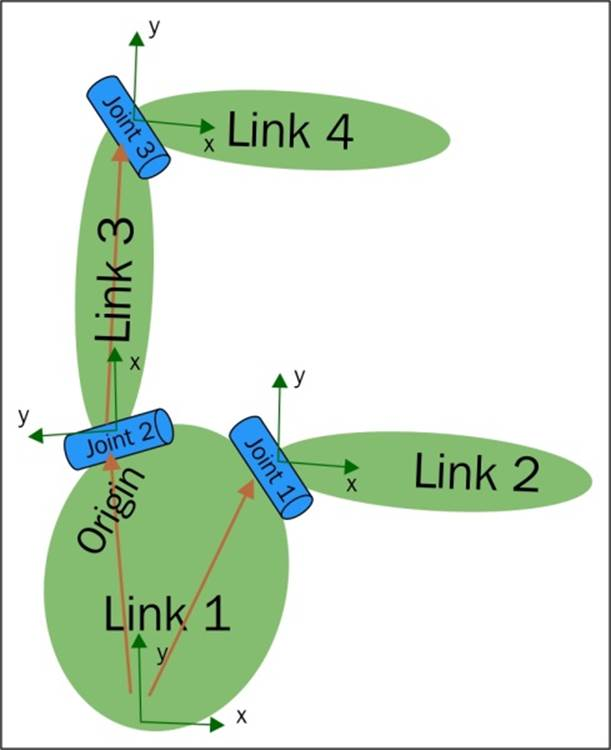
\includegraphics[width=0.7\linewidth]{s3}
	\caption{Visualization of a robot model having joints and links}
	\label{fig:s3}
\end{figure}

\section{Creating our URDF model}
To start first we create the urdf file, let's call it\textit{ zaghexasim.urdf} and put in
the following code; this URDF code is based on XML.As you will see in the code, there are two principal fields that describe the geometry of a robot: links and joints.\\
the first link has the name base link; this name must be unique to the file\\
\begin{lstlisting}[language=XML]
<?xml version="1.0" ?>
<robot name="zaghexa" xmlns:xacro="http://ros.org/wiki/xacro">
 <!-- Build the body frame -->
<link name="base_link"/>
<joint name="base_joint" type="fixed">
<parent link="base_link"/>
<child link="box"/>
<origin rpy="0 0 0" xyz="0 0 0"/>
</joint>
<link name="box">
<visual>
<origin rpy="0 0 0" xyz="0 0 0"/>
<geometry>
<mesh filename="package://zaghexa_sim/meshes/box.STL"/>
</geometry>
<material name="grey">
<color rgba="0.5 0.5 0.5 1"/>
</material>
</visual>
</link>
\end{lstlisting}
In the joint field we define the name which must be unique as well also we define 
the type of joint(fixed,revolute,continous,floating or planar) the parent, and the child.\\
in our case tibia,femur and leg centre joint are the children of base link which is fixed but all of other joints are revolute.\\
\textbf{this is a sample of one leg and how does it build}\\
\begin{lstlisting}[language=XML]
<!-- Joint properties -->
<!-- Leg macros -->
<!-- Build robot model -->
<joint name="leg_center_joint_r1" type="fixed">
<origin rpy="0 0 0" xyz="0.087598 -0.050575 0"/>
<parent link="box"/>
<child link="leg_center_r1"/>
</joint>
<link name="leg_center_r1"/>
<joint name="coxa_joint_r1" type="revolute">
<origin rpy="0 0 -1.0471975512" xyz="0 0 0"/>
<parent link="leg_center_r1"/>
<child link="coxa_r1"/>
<axis xyz="0 0 -1"/>
<limit effort="10000" lower="-1.5" upper="1.5" velocity="100"/>
</joint>
<link name="coxa_r1">
<visual>
<origin rpy="0 0 0" xyz="0 0 0"/>
<geometry>
<mesh filename="package://zaghexa_sim/meshes/coxa_r.STL"/>
</geometry>
<material name="">
<color rgba="0.7 0.7 0 1"/>
</material>
</visual>
</link>
<joint name="femur_joint_r1" type="revolute">
<origin rpy="-1.57079632679 0 0" xyz="0.0294 0 0"/>
<parent link="coxa_r1"/>
<child link="zaghexa"/>
<axis xyz="0 0 -1"/>
<limit effort="10000" lower="-1.5" upper="1.5" velocity="100"/>
</joint>
<link name="zaghexa">
<visual>
<origin rpy="0 0 0" xyz="0 0 0"/>
<geometry>
<mesh filename="package://zaghexa_sim/meshes/femur_r.STL"/>
</geometry>
<material name="">
<color rgba="0 0.7 0.7 1"/>
</material>
</visual>
</link>
<joint name="tibia_joint_r1" type="revolute">
<origin rpy="3.14159265359 0 1.57079632679" xyz="0.08 0 0"/>
<parent link="zaghexa"/>
<child link="tibia_r1"/>
<axis xyz="0 0 1"/>
<limit effort="10000" lower="-1.5" upper="1.5" velocity="100"/>
</joint>
<link name="tibia_r1">
\end{lstlisting}
\textbf{You can check the syntax of the urdf whether we have errors, we can use:
check urdf command tool:}
\begin{lstlisting}[language=terCmd]
$ rosrun urdf_parser check_urdf zaghexa_sim.urdf
\end{lstlisting}

If you want to see it graphically, you can use the urdf to graphiz command tool
\begin{lstlisting}[language=terCmd]
$ rosrun urdf_parser urdf_to_graphiz "`rospack find zaghexa_sim`/urdf/zaghexa_sim.urdf"
\end{lstlisting}
\textbf{The following is what you will receive as output:}
\begin{figure}[hbt]
    \centering
    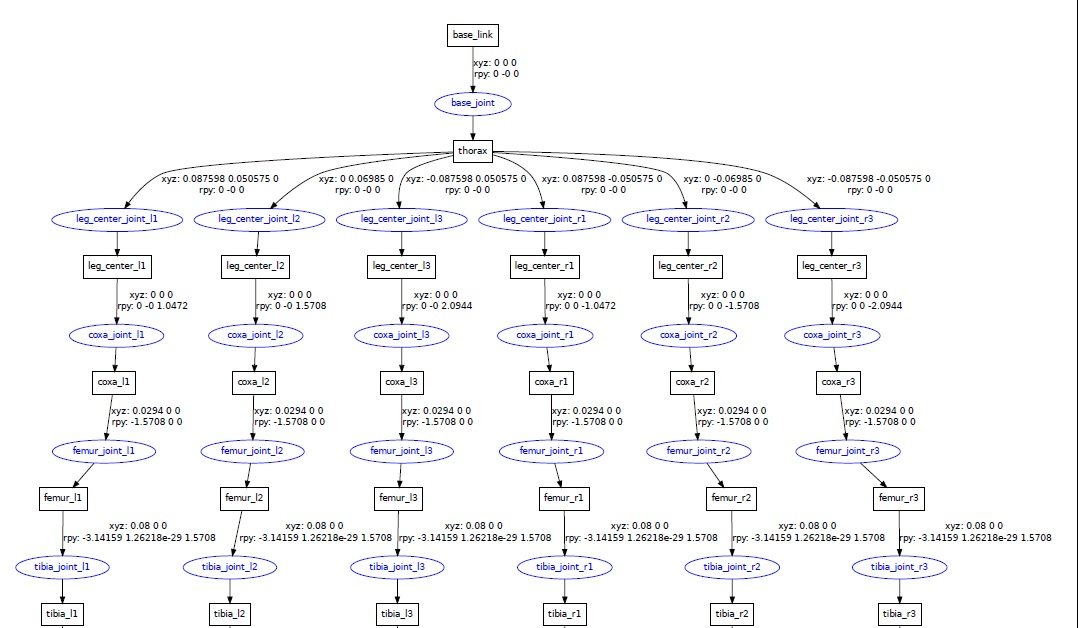
\includegraphics[width=\linewidth, height=0.5\textheight]{s4}
    \caption{output of urdf to graphics}
    \label{figure :s4}
\end{figure}

\section{Watching the 3D model in RVIZ}
Now that we have the model of our robot, we can use it on rviz to watch it in 3D
and see the movements of the joints.\\
We will create the display.launch file in zaghexa-sim/launch folder,
and put the following code in it:
\begin{lstlisting}[language=XML]
>>>>>>> origin/master
	<launch>
	<arg
	name="model" />
	<arg
	name="gui"
	default="True" />
	<param
	name="robot_description"
	command="$(find xacro)/xacro.py '$(find zaghexa_sim)/models/zaghexa_model.xacro'" />
	<param
	name="use_gui"
	value="$(arg gui)" />
	<param
	name="rate"
	value="25" />
	<rosparam param="source_list">
	[leg_joints_states]
	</rosparam>
	<node
	name="joint_state_publisher"
	pkg="joint_state_publisher"
	type="joint_state_publisher" />
	<node
	name="robot_state_publisher"
	pkg="robot_state_publisher"
	type="state_publisher" />
	<node
	name="rviz"
	pkg="rviz"
	type="rviz"
	args="-d $(find zaghexa_sim)/urdf.rviz" />
	</launch>
<<<<<<< HEAD
	\end{lstlisting}	
	\textbf{We will launch it with the following command:}
	\begin{lstlisting}
	$ roslaunch zaghexa_sim display_model.launch model:="`rospack find
	zaghexa_sim`/urdf/zaghexa_sim.urdf"
	\end{lstlisting}
	\textbf{if every thing is fine and you have no errors, it will load RVIZ and you will see:}
	\begin{figure}[h]
		\centering
		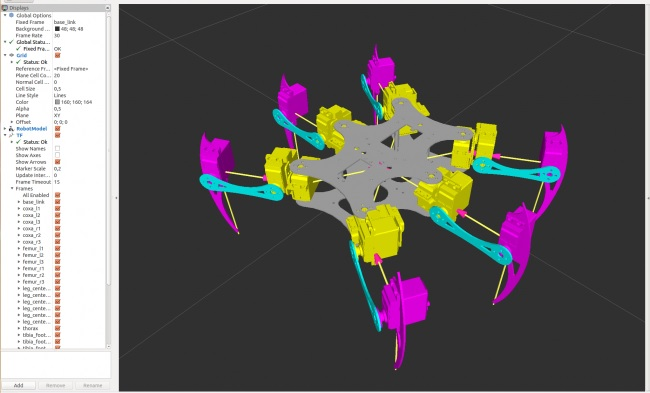
\includegraphics[width=1\linewidth, height=0.26\textheight]{s5}
		\caption{output of urdf to graphics}
		\label{figure :s5}
	\end{figure}
	\subsection{Making our robot movable}
	\textbf{A good way of testing whether or not the axis and limits of the joints are fine by running rviz with joint state publisher GUI}
	\begin{lstlisting}
	$ roslaunch zaghexa_sim display.launch model:="`rospack find
	zaghexa_sim`/urdf/zaghexa_sim.urdf" gui:=true
	
	\end{lstlisting}
	\textbf{you will see a GUI with some sliders each of them controls one joint of the 18 joints so we have 18 sliders:}
	\begin{figure}[h]
		\centering
		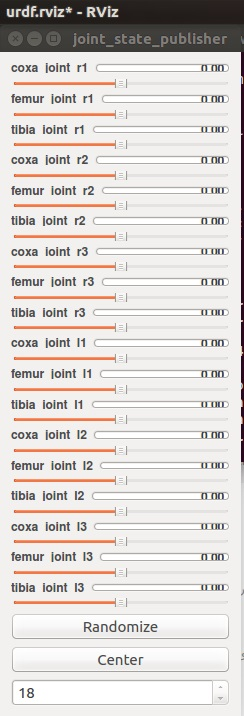
\includegraphics[height=0.3\textheight]{s6}
		\caption{Joint state publisher GUI}
		\label{fig:s6}
	\end{figure}
	\\\textbf{In the next figures you will see the effect of changing sliders values to the joints angles and positions}
	\begin{figure}[h]
		\centering
		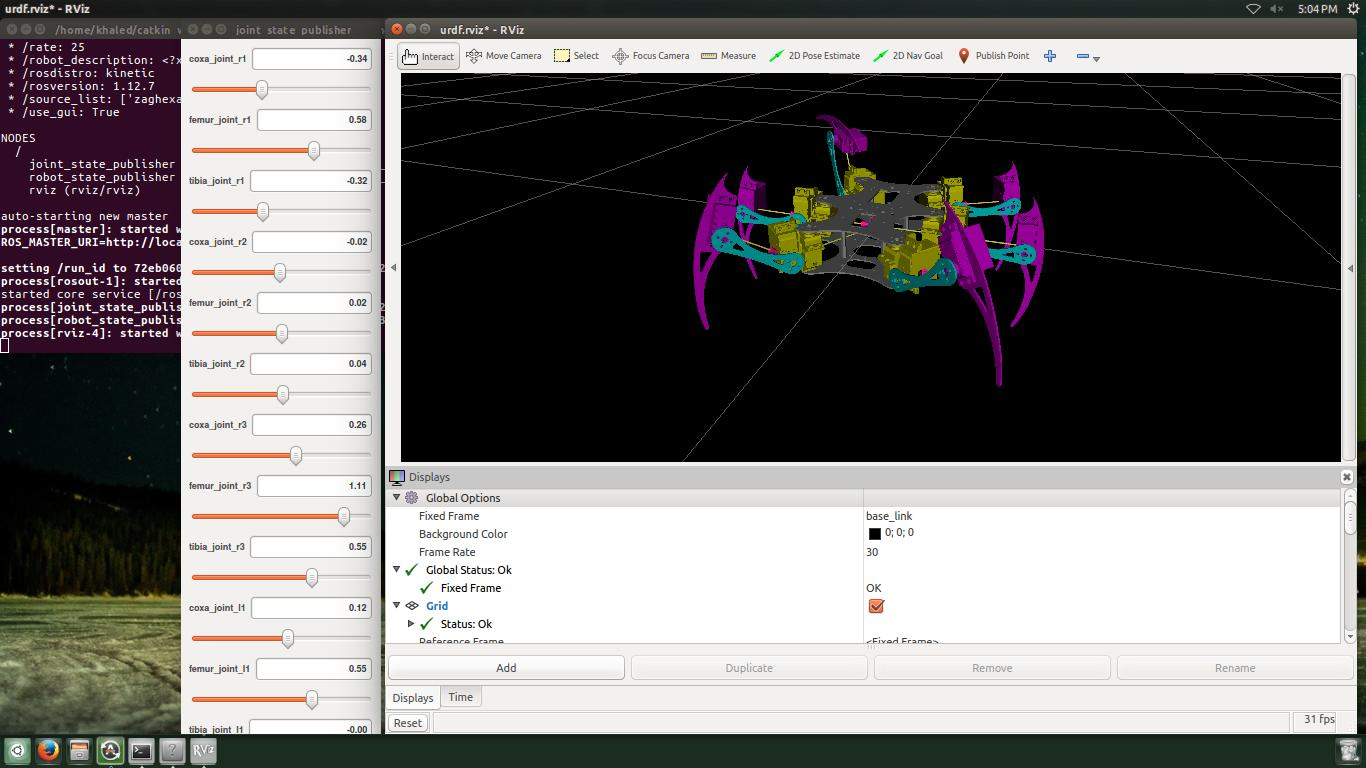
\includegraphics[height=.5\linewidth]{s7}
		\caption{Control sliders and their effect on the robot }
		\label{fig:s7}
	\end{figure}
	\begin{figure}[htb]
		\centering
		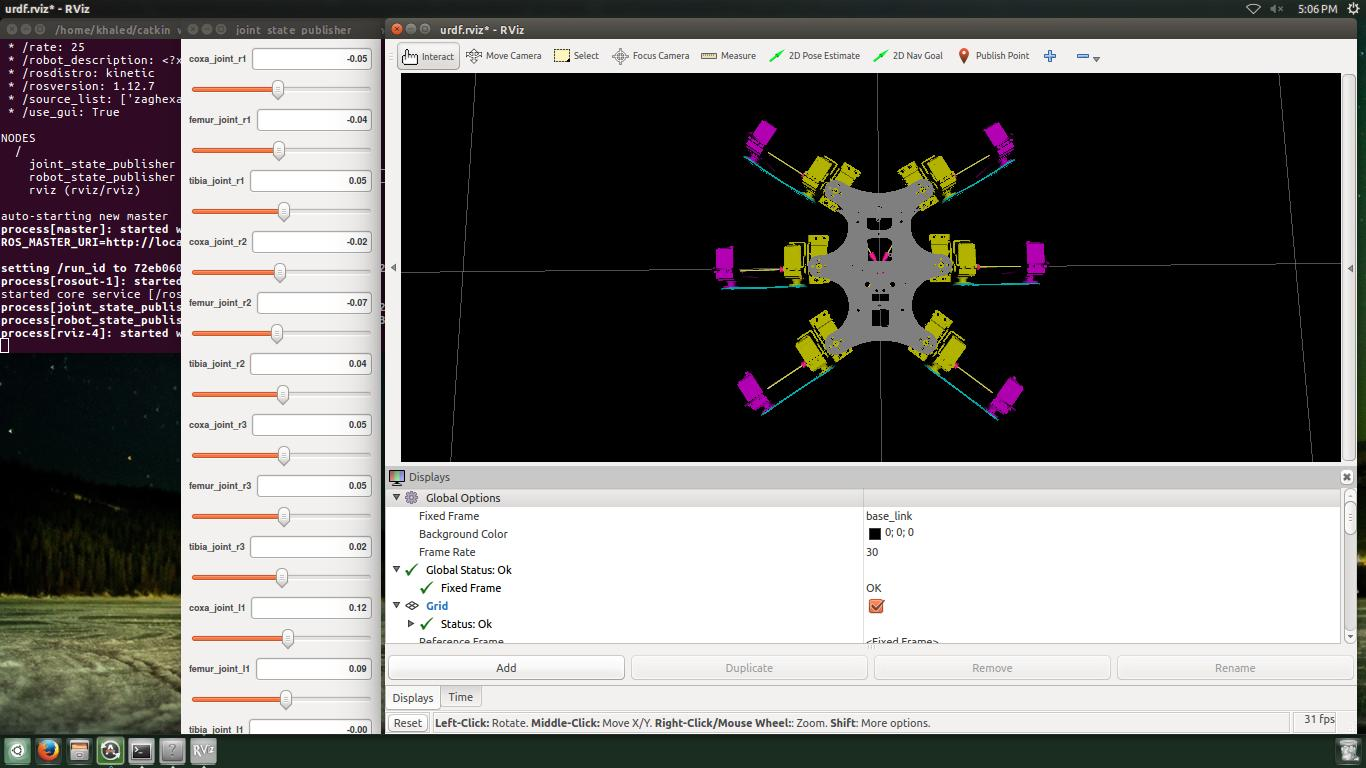
\includegraphics[height=0.5\linewidth]{s8}
		\caption{top view of the robot}
		\label{fig:s8}
		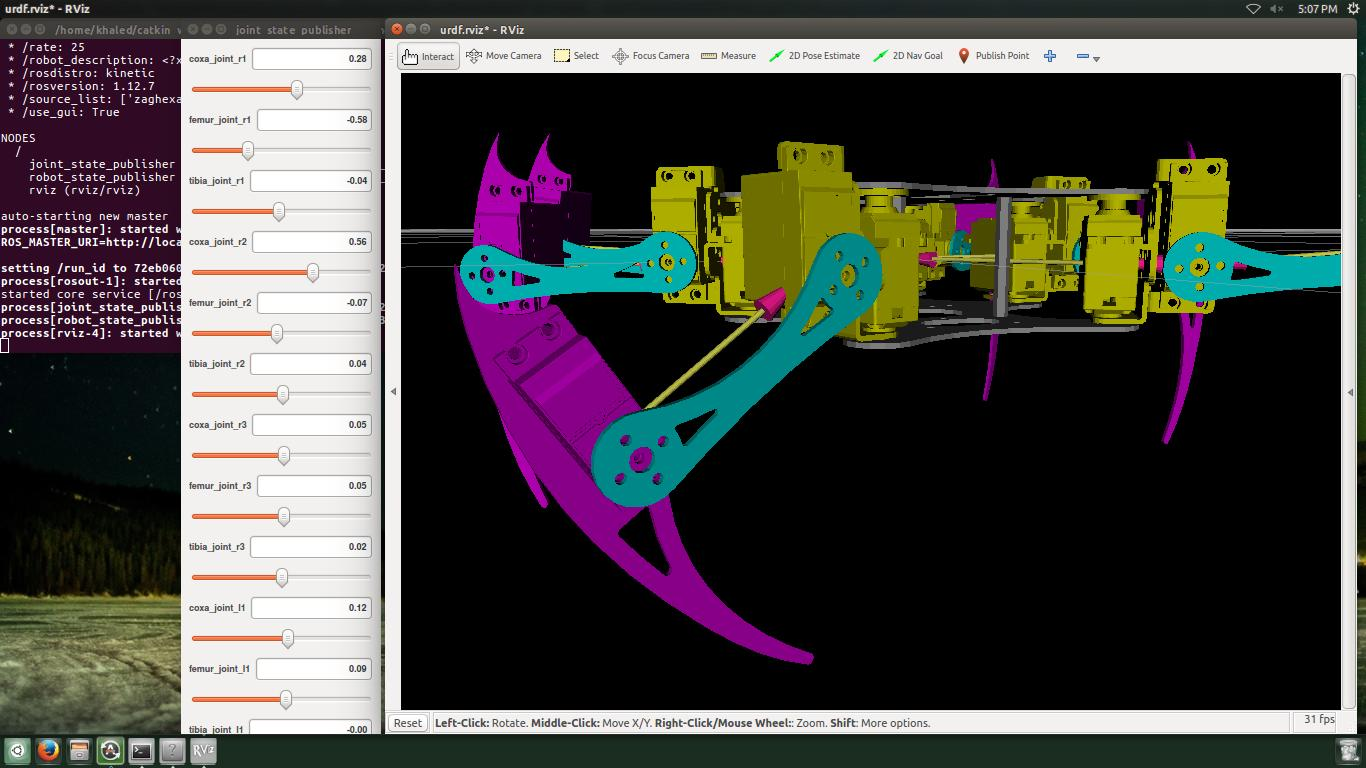
\includegraphics[height=0.5\linewidth]{s9}
		\caption{Different views of the robot}
		\label{fig:s9}
		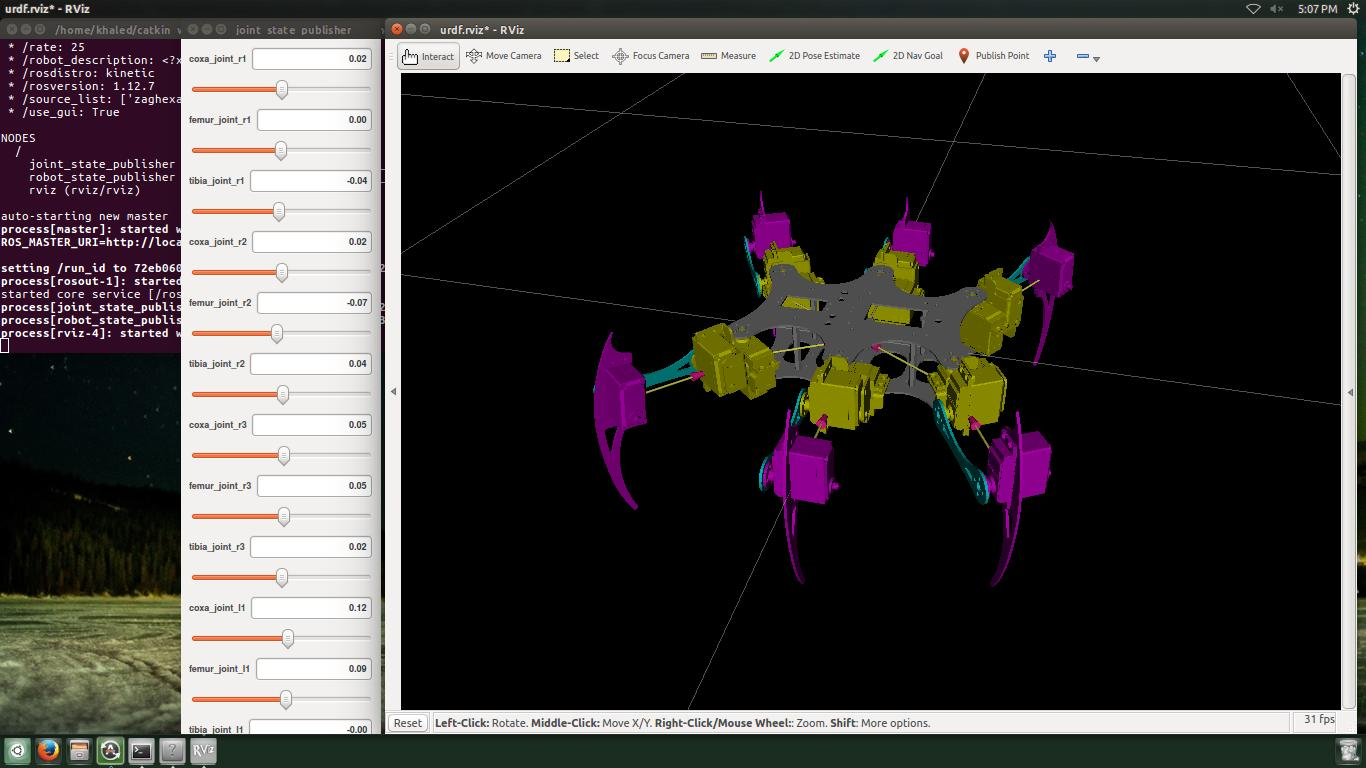
\includegraphics[height=0.5\linewidth]{s10}
		\caption{Different views of the robot}
		\label{fig:s10}
	\end{figure}
\clearpage
\vspace{10cm}
\section{ Matlab Simulation}
In the second simulation, we modelled the robot in MATLAB and employing the Robotics Toolbox. The main purpose of this simulation is to calculate and simulate the kinematics of robot. To create the six-legged walking robot, we started by creating a three-axis robot arm that we used as a leg. Then we implemented a trajectory for the leg that is suitable for walking. Finally, we instantiated six instances of the leg to create the walking robot. The equations given in Sec.4 are programmed first for one leg and tested on successful working, the whole body kinematics were also programmed and tested.
The results were very useful in modifying the walking gaits of the robot which then implemented in the real robot. Figure 10 shows one such simulations in which the same experiment performed on the real robot to test the whole body kinematics for raising and lowering the body height.
\begin{figure}[h]
	\centering
	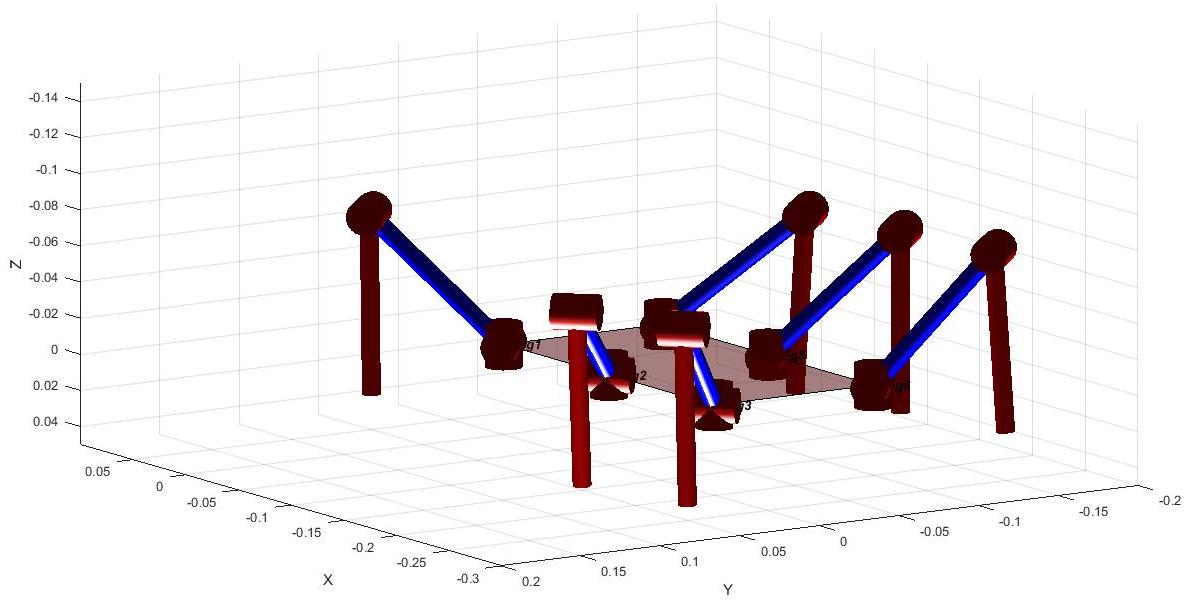
\includegraphics[width =.8\textwidth]{Fig15_1.jpg} 
	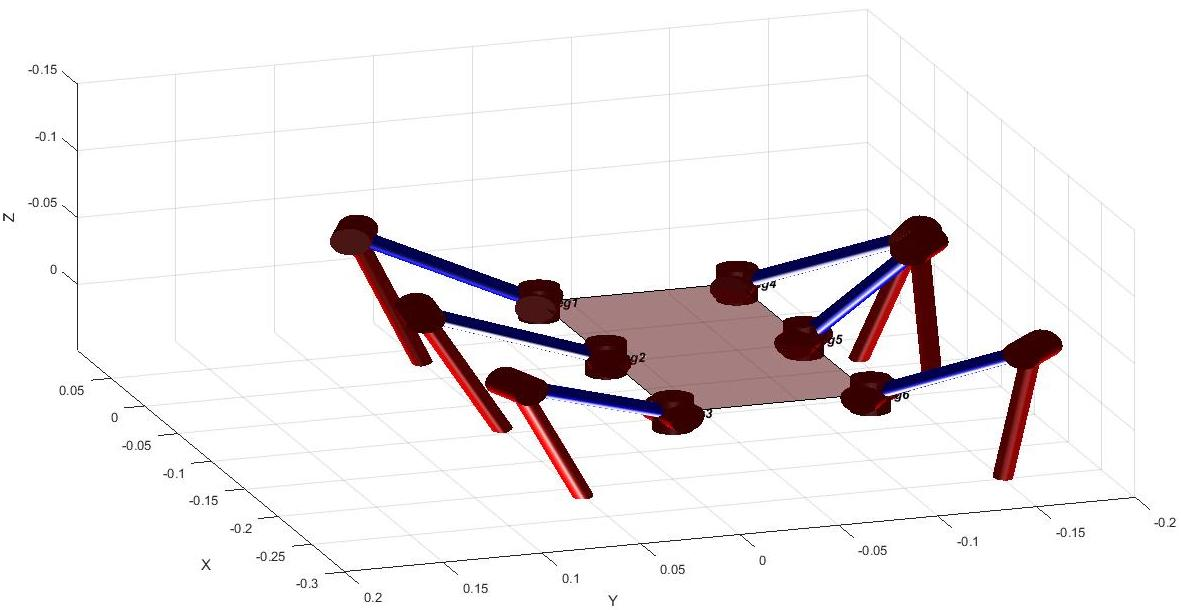
\includegraphics[width =.8\textwidth]{Fig15_2.jpg}
	\caption{ Hexapod robot Simulation.}
	\label{sim}
\end{figure}

\textbf{We will launch it with the following command:}
\begin{lstlisting}[language=terCmd]
$ roslaunch zaghexa_sim display_model.launch model:="`rospack find zaghexa_sim`/urdf/zaghexa_sim.urdf"
\end{lstlisting}

\textbf{if every thing is fine and you have no errors, it will load RVIZ and you will see:}
\begin{figure}[h]
	\centering
	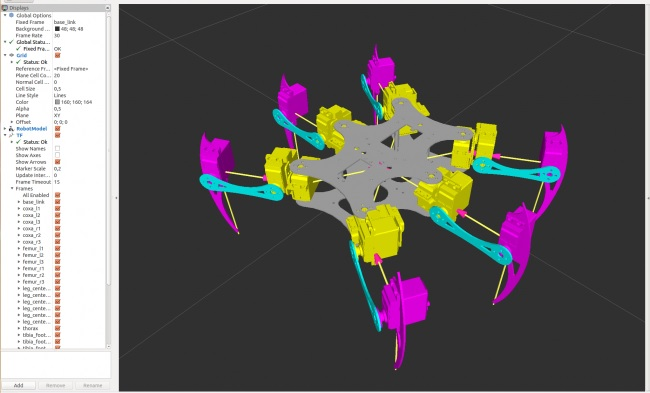
\includegraphics[width=\linewidth, height=0.4\textheight]{s5}
	\caption{output of urdf to graphics}
	\label{figure :s5}
\end{figure}

\section{Making our robot movable}
\textbf{A good way of testing whether or not the axis and limits of the joints are fine by running rviz with joint state publisher GUI}
\begin{lstlisting}[language=terCmd]
$ roslaunch zaghexa_sim display.launch model:="`rospack find zaghexa_sim`/urdf/zaghexa_sim.urdf" gui:=true
\end{lstlisting}


\textbf{you will see a GUI with some sliders each of them controls one joint of the 18 joints so we have 18 sliders:}
%\begin{figure}[h]
%	\centering
%	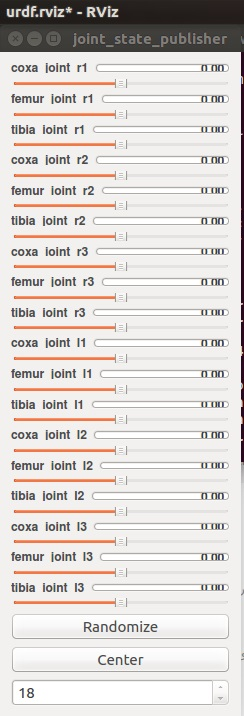
\includegraphics[height=0.3\textheight]{s6}
%	\caption{Joint state publisher GUI}
%	\label{fig:s6}
%\end{figure}
\\\textbf{In the next figures you will see the effect of changing sliders values to the joints angles and positions}
\begin{figure}[h]
	\centering
	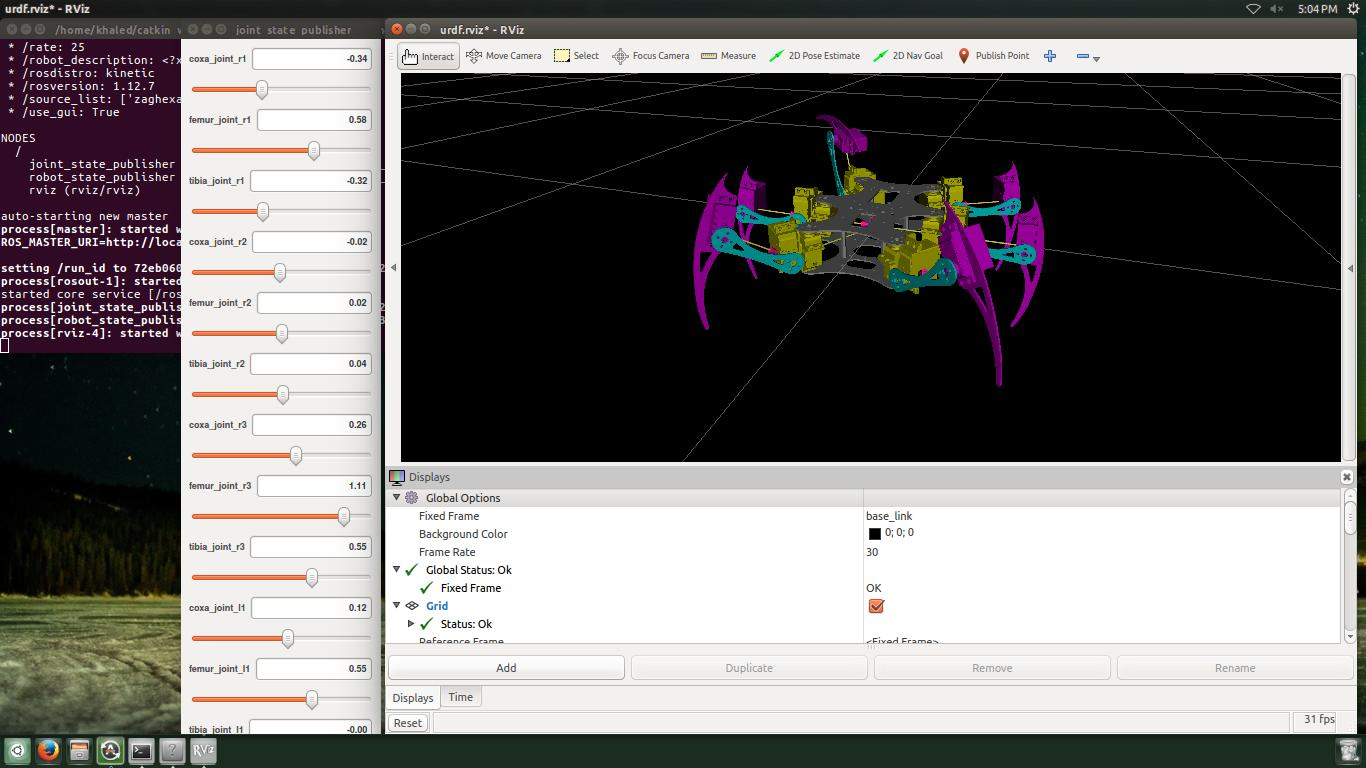
\includegraphics[width=\textwidth]{s7}
	\caption{Joint state publisher GUI with its control sliders and their effect on the robot }
	\label{fig:s7}
\end{figure}
\begin{figure}[htb]
	\centering
	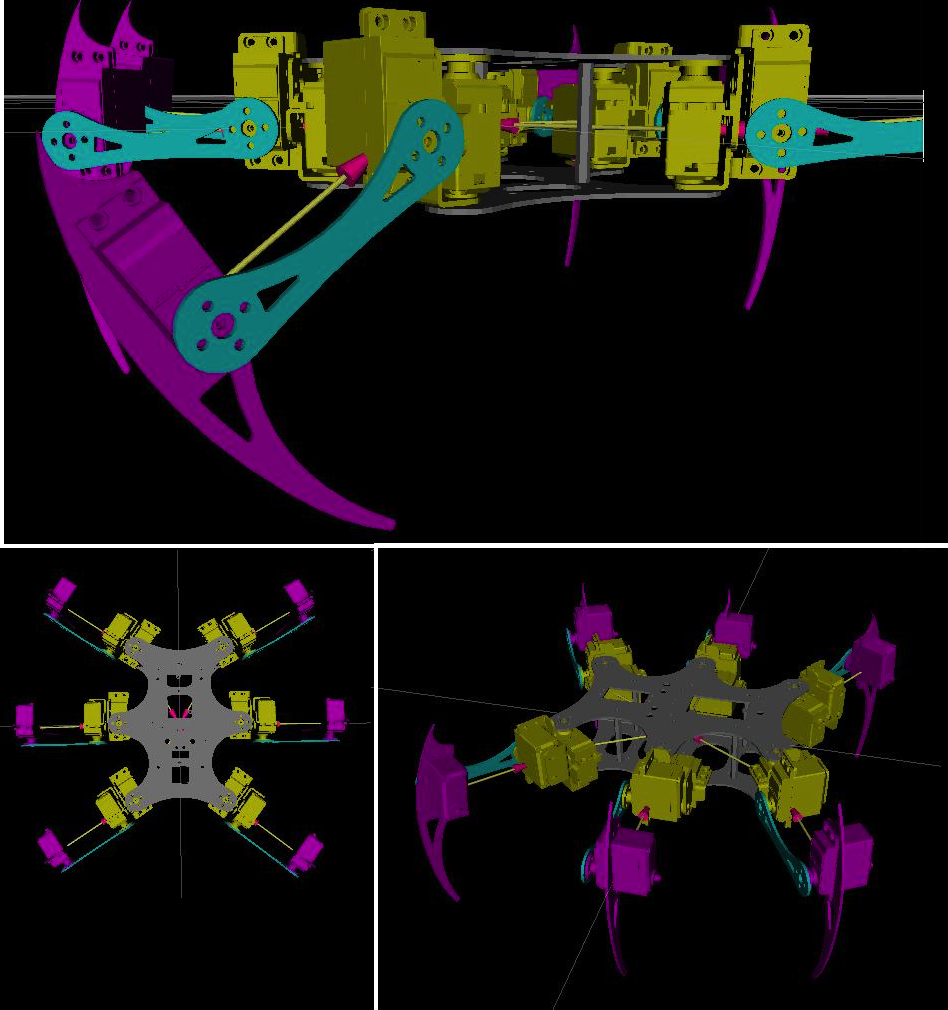
\includegraphics[width=0.6\textwidth]{simViews}
    	\caption{Different views of the robot}
%	\caption{top view of the robot}
%	\label{fig:s8}
%	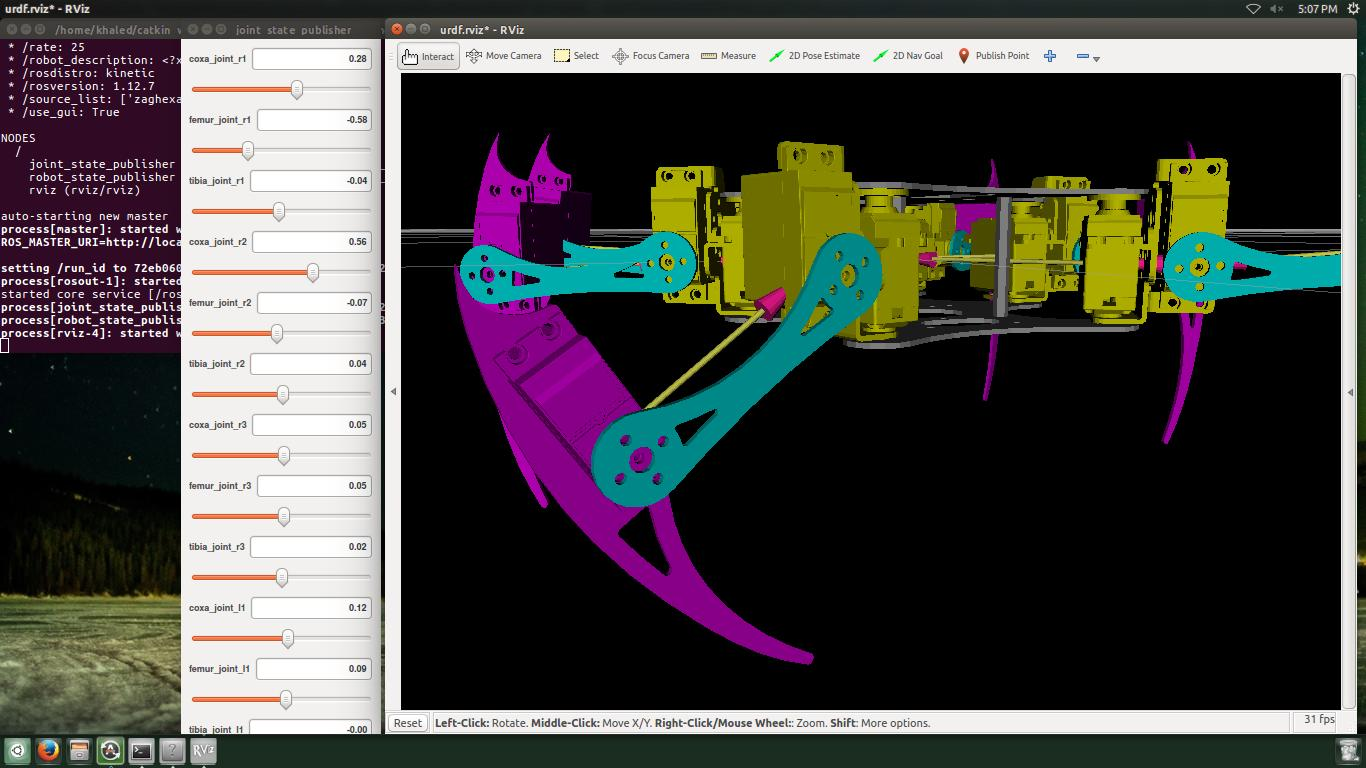
\includegraphics[height=0.3\textheight]{s9}
%	\caption{Different views of the robot}
%	\label{fig:s9}
%	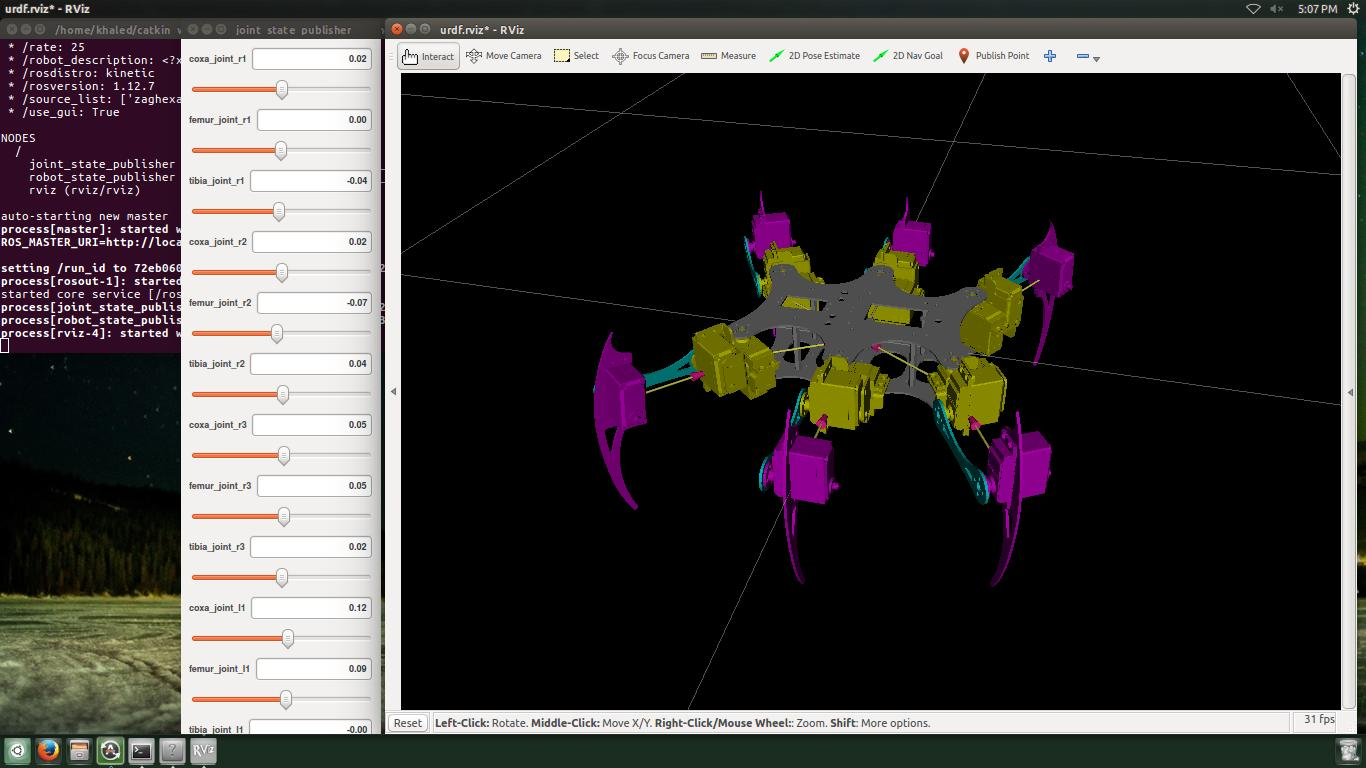
\includegraphics[height=0.3\textheight]{s10}
%	\caption{Different views of the robot}
%	\label{fig:s10}
\end{figure}